\documentclass{article}
\usepackage[utf8]{inputenc}
\usepackage{amsmath}
\usepackage{multirow}
\usepackage[inline]{enumitem}
\usepackage{graphicx}
\graphicspath{ {./images/} }
\newcommand{\lt}{\latintext}
\newcommand{\gt}{\greektext}

\usepackage{tikz}
\usepackage{pgfplots}

\pgfplotsset{compat = newest}

\title{\gt \textbf{Πρώτη Υποχρεωτική Εργασία}}
\author{\gt \LargeΟνοματεπώνυμο: Ασημάκης Κύδρος \\ ΑΕΜ: 3881}
\date{\gt \Large26 Δεκεμβρίου 2021}

%%Activate Greek ASCII characters
\usepackage[english,greek]{babel}

\begin{document}
\maketitle

\pagebreak
%%---------ΠΡΩΤΗ ΑΣΚΗΣΗ---------
\section{\gt Πρώτη Άσκηση}
\Large
\gt Έχουμε να βρούμε τις ρίζες της παρακάτω συνάρτησης:\\
\begin{equation*}
    f(x) = 14xe^{x - 2} - 12e^{x - 2} - 7x^{3} + 20x^{2} - 26x + 12,\quad x\epsilon[0,3]
\end{equation*}
\begin{center}
    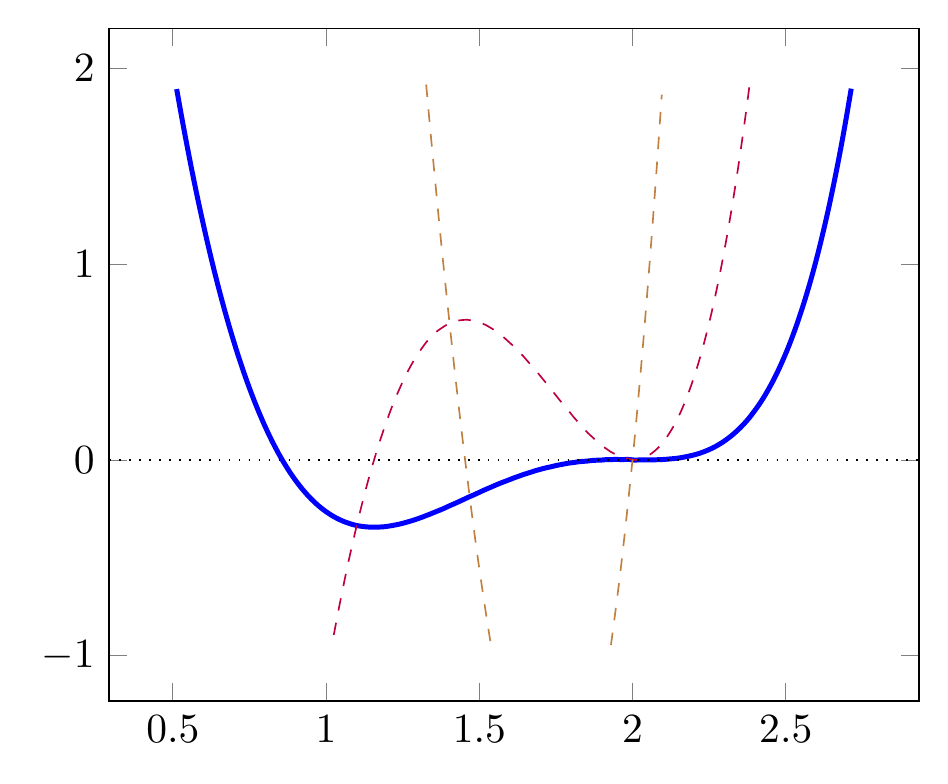
\begin{tikzpicture}[scale = 1.5]
        \begin{axis} [
            domain = 0:3,
            restrict y to domain = -1:2
        ]
        %%function F
            \addplot[
                domain = 0:3,
                samples = 200,
                smooth,
                very thick,
                blue,
            ] {
                14*x*exp(x-2) - 12*exp(x-2) - 7*x^3 + 20*x^2 - 26*x + 12
            };
        %%function F'
            \addplot[
                domain = 0:3,
                samples = 200,
                smooth,
                thin,
                purple,
                dashed
            ] {
                14*x*exp(x-2) + 2*exp(x-2) - 21*x^2 + 40*x - 26
            };
            \draw[
                dotted
            ]
            (0, 0) -- (3,0);
        %%function F''
            \addplot[
                domain = 0:3,
                samples = 200,
                smooth,
                thin,
                brown,
                dashed
            ] {
                14*x*exp(x-2) + 16*exp(x-2) - 42*x + 40
            };
            \draw[
                dotted
            ]
            (0, 0) -- (3,0);
        \end{axis}
    \end{tikzpicture}
\end{center}
\gt το γράφημα της \lt f\gt , με τις διακεκομμένες να παριστάνουν τις \lt f', f''.\\
\gt (Αναλυτικότερα γραφήματα σε \lt GeoGebra \gtστον αντίστοιχο φάκελο στο \lt.rar)\\
\newpage
\gt Παρατηρούμε ότι οι θέσεις των ριζών είναι 2, άρα οι ρίζες είναι τουλάχιστον 2.
\gt Θα χρησιμοποιήσουμε επαναληπτικές μεθόδους για την προσέγγιση των ριζών αυτών.
\begin{itemize}
    \item \textbf{\gtΜέθοδος της διχοτόμησης:}\\
            \gtΗ μέθοδος απαιτεί διαστήματα όπου ικανοποιείται το θεώρημα \lt Bolzano,
            \gtεπομένως σπάμε το πεδίο ορισμού σε [0,1], [1.5,3] και έχουμε:\\
            \lt x ~= 0.85714 \gtσε 19 επαναλήψεις\\
            \lt x ~= 2.00001 \gtσε 20 επαναλήψεις
    \item \textbf{\gtΜέθοδος \lt Newton-Raphson:}\\
            \gtΜε την ίδια λογική χρησιμοποιούμε τα ίδια υποδιαστήματα και έχουμε:\\
            \lt x ~= 0.85714 \gtσε 7 επαναλήψεις\\
            \lt x ~= 1.99999 \gtσε 26 επαναλήψεις
    \item \textbf{\gtΜέθοδος της τέμνουσας:}\\
            \gtΓια ακόμα μια φορά παίρνουμε τα παραπάνω υποδιαστήματα και έχουμε:\\
            \lt x ~= 0.85714 \gtσε 7 επαναλήψεις\\
            \lt x ~= 1.99999 \gtσε 38 επαναλήψεις
\end{itemize}

\gtΤο υποδιάστημα [1,1.5] αγνοείται γιατί γνωρίζουμε από το γράφημα ότι εκεί
\gtδεν υπάρχει ρίζα της \lt f \gtκαι επίσης στο [0,1] ισχύει η προϋπόθεση σύγκλισης των
\lt Newton-Raphson \gt(άρα και της τέμνουσας), δηλαδή
\begin{equation*}
    \lt f',f'' \neq 0
\end{equation*}

\gtΓια την πρώτη ρίζα, γίνεται προφανής η τεράστια υπεροχή των \lt N-R \gtκαι τέμνουσας
\gtσε θέματα ταχύτητας. Στην δέυτερη όμως, οι μέθοδοι αυτοί φαίνεται να δυσκολέυονται, αν και
\gtσυγκριτικά μεταξύ τους η \lt Newton-Raphson \gtδιατηρεί την υπεροχή της. Αυτό συμβαίνει γιατί
\gtη \lt N-R \gt(και άρα και η τέμνουσα) συγκλίνει τετραγωνικά για την 0.85714 αλλά όχι για την 2,
\gtκάτι αναμενόμενο καθώς από το διάγραμμα φαίνεται οτι η 2 είναι τριπλή ρίζα της \lt f,
\gtάρα:
\begin{equation*}
    \lim_{x \to \infty} \frac{x_{n+1} - 2}{(x_n - 2)^{2}} = \frac{f^{''}(2)}{2f^{'}(2)}\not\in R \quad (\frac{0}{0})
\end{equation*}
\gtκαι επομένως δεν συγκλίνει τετραγωνικά.

\newpage
%%---------ΔΕΥΤΕΡΗ ΑΣΚΗΣΗ---------
\section{\gt Δεύτερη Άσκηση}
\gtΈχουμε να βρούμε τις ρίζες της παρακάτω συνάρτησης:
\begin{equation*}
    f(x) = 54x^{6} + 45x^{5} - 102x^{4} - 69x^{3} + 35x^{2} + 16x - 4, \quad x\epsilon[-2,2]
\end{equation*}
\begin{center}
    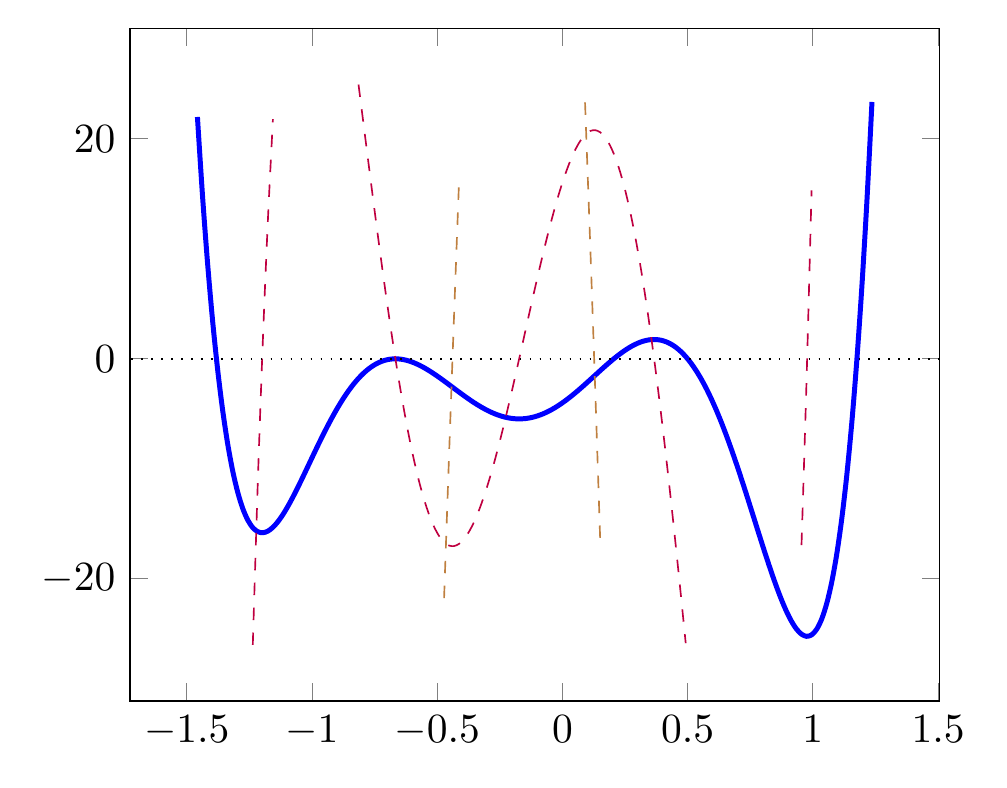
\begin{tikzpicture}[scale = 1.5]
        \begin{axis} [
            domain = -2:2,
            restrict y to domain = -27:27
        ]
        %%function F
            \addplot[
                domain = -2:2,
                samples = 200,
                smooth,
                very thick,
                blue,
            ] {
                54*x^6 + 45*x^5 - 102*x^4 - 69*x^3 + 35*x^2 + 16*x - 4
            };
            %%function F'
            \addplot[
                domain = -2:2,
                samples = 200,
                smooth,
                thin,
                purple,
                dashed
            ] {
                6*54*x^5 + 5*45*x^4 - 4*102*x^3 - 3*69*x^2 + 35*2*x + 16
            };
            \draw[
                dotted
            ]
            (-2, 0) -- (2,0);
        %%function F''
            \addplot[
                domain = -2:2,
                samples = 200,
                smooth,
                thin,
                brown,
                dashed
            ] {
                30*54*x^4 + 20*45*x^3 - 12*102*x^2 - 6*69*x + 70
            };
            \draw[
                dotted
            ]
            (-2, 0) -- (2,0);
        \end{axis}
    \end{tikzpicture}
\end{center}
\gt το γράφημα της \lt f\gt , με τις διακεκομμένες να παριστάνουν τις \lt f', f''.\\
\gt (Αναλυτικότερα γραφήματα σε \lt GeoGebra \gtστον αντίστοιχο φάκελο στο \lt.rar)\\
\newpage
%%ΠΡΩΤΟ ΖΗΤΟΥΜΕΝΟ ΑΣΚΗΣΗΣ 2
\textbf{\gt Ζητούμενο 1)}\\
\gtΘα χρησιμοποιήσουμε τις παραλλαγμένες επαναληπτικές μεθόδους για την έυρεση των ριζών της.
\gtΠαρατηρούμε ωστόσο ότι η ρίζα στο διάστημα [-0.8,-0.4] έιναι απροσέγγιστη με όλες τις μεθόδους,
\gtκαθώς δεν υπάρχει υποδιάστημα που να την περιέχει στο οποίο να ικανοποιούνται οι προϋποθέσεις
\gtτου θεωρήματος \lt Bolzano.
\begin{itemize}
    \item \textbf{\lt Randomized \gtμέθοδος διχοτόμησης:}\\
            \gtΠαρ'όλο παραλλαγμένες, όλες οι μέθοδοι συνεχίζουν να απαιτούν να ικανοποιείται το
            \gt θ.\lt Bolzano \gt στα διαστήματα που μελετούν. Επομένως σπάμε το πεδίο ορισμού στα
            \gt[-2,-1.3], [0.15,0.3], [0.4,0.7], [1,1.5], προκειμένου να ισχύουν και οι προϋποθέσεις
            \gtσύγκλισης της \lt N-R,\gt και έχουμε:\\
            \lt x = -1.38130 \gt σε 30 επαναλήψεις\\
            \lt x = 0.20518 \gt σε 20 επαναλήψεις\\
            \lt x = 0.49999 \gt σε 22 επαναλήψεις\\
            \lt x = 1.17610 \gt σε 18 επαναλήψεις\\
    \item \textbf{\gt Παραλλαγμένη μέθοδος \lt Newton-Raphson:}\\
            \gtΧρησιμοποιώντας τα παραπάνω υποδιαστήματα:\\
            \lt x = -1.38130 \gt σε 5 επαναλήψεις\\
            \lt x = 0.20518 \gt σε 3 επαναλήψεις\\
            \lt x = 0.50000 \gt σε 4 επαναλήψεις\\
            \lt x = 1.17612 \gt σε 4 επαναλήψεις\\
    \item \textbf{\gt Παραλλαγμένη μέθοδος τέμνουσας:}\\
            \gtΧρησιμοποιώντας τα παραπάνω υποδιαστήματα:\\
            \lt x = -1.38130 \gt σε 6 επαναλήψεις\\
            \lt x = 0.20518 \gt σε 4 επαναλήψεις\\
            \lt x = 0.50000 \gt σε 5 επαναλήψεις\\
            \lt x = 1.17612 \gt σε 6 επαναλήψεις\\
\end{itemize}

%%ΔΕΥΤΕΡΟ ΖΗΤΟΥΜΕΝΟ ΑΣΚΗΣΗΣ 2
\textbf{\gt Ζητούμενο 2)}\\
\gtΤρέχοντας τον αλγόριθμο της \lt randomized bisection \gt10 φορές για την ίδια ριζα βλέπουμε πως
\begin{center}
    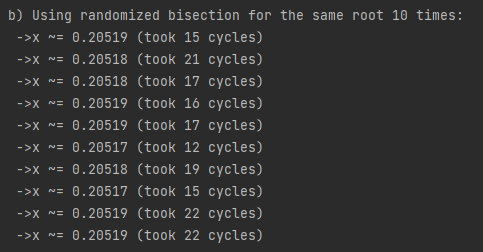
\includegraphics[scale=0.7]{images/output of question 2.png}        
\end{center}
\gtδεν συγκλίνει πάντα σε ίδιο αριθμό επαναλήψεων.\\

%%ΤΡΙΤΟ ΖΗΤΟΥΜΕΝΟ ΑΣΚΗΣΗΣ 2
\textbf{\gt Ζητούμενο 3)}\\
\gtΧρησιμοποιούμε τις κανονικές μεθόδους για την εύρεση των ίδιων ριζών:
\begin{itemize}
    \item \textbf{\gtΜέθοδος διχοτόμησης:}\\
            \gtΧρησιμοποιώντας τα παραπάνω υποδιαστήματα:\\
            \lt x = -1.38130 \gt σε 19 επαναλήψεις\\
            \lt x = 0.20518 \gt σε 16 επαναλήψεις\\
            \lt x = 0.50000 \gt σε 17 επαναλήψεις\\
            \lt x = 1.17612 \gt σε 18 επαναλήψεις\\
    \item \textbf{\gtΜέθοδος \lt Newton-Raphson:}\\
            \gtΧρησιμοποιώντας τα παραπάνω υποδιαστήματα:\\
            \lt x = -1.38130 \gt σε 8 επαναλήψεις\\
            \lt x = 0.20518 \gt σε 4 επαναλήψεις\\
            \lt x = 0.50000 \gt σε 5 επαναλήψεις\\
            \lt x = 1.17612 \gt σε 6 επαναλήψεις\\
    \item \textbf{\gtΜέθοδος τέμνουσας:}\\
            \gtΧρησιμοποιώντας τα παραπάνω υποδιαστήματα:\\
            \lt x = -1.38130 \gt σε 7 επαναλήψεις\\
            \lt x = 0.20518 \gt σε 5 επαναλήψεις\\
            \lt x = 0.50000 \gt σε 7 επαναλήψεις\\
            \lt x = 1.17612 \gt σε 10 επαναλήψεις\\
\end{itemize}

\gtΑπό τα παραπάνω φαίνεται πώς οι τροποποιημένες μέθοδοι \lt Newton-Raphson \gt και τέμνουσας
\gt τείνουν να είναι γρηγορότερες, ενώ η τυχαία μέθοδος διχοτόμησης είναι συντρηπτικά χειρότερη
\gt από την κανονική.

\newpage
%%---------ΤΡΙΤΗ ΑΣΚΗΣΗ---------
\section{\gt Τρίτη Άσκηση}
\gt Παρατηρούμε πως ο δοθήσας πίνακας Α ικανοποιεί τις προϋποθέσεις όλων των ζητούμενων μεθόδων,
\gt για κάθε μήκος πλευράς \lt n. \gt Για παράδειγμα, για \lt n = 5:
\begin{enumerate}
    \item \textbf{\gt είναι τετραγωνικός}
    \begin{equation*}
        \textbf{A} = 
        \begin{bmatrix}
            5 & -2 & 0 & 0 & 0\\
            -2 & 5 & -2 & 0 & 0\\
            0 & -2 & 5 & -2 & 0\\
            0 & 0 & -2 & 5 & -2\\
            0 & 0 & 0 & -2 & 5
        \end{bmatrix}
    \end{equation*}
    \item \textbf{\gt είναι συμμετρικός}\\
            \gt καθώς φαίνεται ότι
            \begin{equation*}
               \lt  A(i,j) = A(j, i), \quad \forall i,j = 0,1,2,3,4\\
            \end{equation*}
    \item \textbf{\gt έχει κυριαρχική διαγώνιο}\\
            \begin{equation*}
                \sum_{j=0,j \neq i}^{4}\left|A(i,j)\right| \leq \left|A(i,i)\right|
                \quad i=0,1,2,3,4
            \end{equation*}\\
    \item \textbf{\gt είναι θετικά ορισμένος}
            \begin{equation*}
                \lt x^{T}Ax = 5(x_1^{2} + x_2^{2} + x_3^{2} + x_4^{2} + x_5^{2}) > 0
                \quad \forall x \in R^{5}
            \end{equation*}
\end{enumerate}
\gt Γνωρίζοντας αυτά, τρέχουμε τις τρεις ζητούμενες συναρτήσεις για τον Α.
\newpage
\begin{itemize}
    \item \textbf{\lt Gauss:}\\
    \begin{equation*}
        \textbf{\lt x} = 
        \begin{bmatrix}
            1 \\
            1 \\
            .\\
            .\\
            .\\
            1 
        \end{bmatrix}
    \end{equation*}
    \item \textbf{\lt Gauss-Seidel:}\\
    \begin{equation*}
        \textbf{\lt x} = 
        \begin{bmatrix}
            0.9999 \\
            0.9999 \\
            .\\
            .\\
            .\\
            0.9999 
        \end{bmatrix}
    \end{equation*}
    \item \textbf{\lt Cholesky \gt του Α} (για \lt n=10):\\
        \begin{center}
            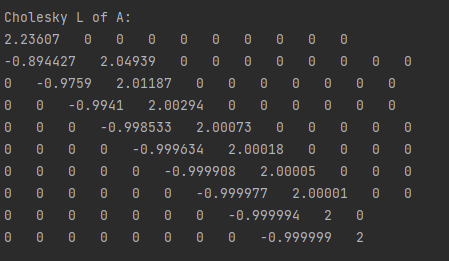
\includegraphics[scale=0.7]{images/cholesky A n=10.png}        
        \end{center}
\end{itemize}

\newpage
%%---------ΤΕΤΑΡΤΗ ΑΣΚΗΣΗ---------
\section{\gt Τέταρτη Άσκηση}
\gt Με βάση τα δεδομένα του πίνακα γειτνίασης και θεωρώντας \lt q = 0.15, \gtαρχικοποιούμε τον
\gt πίνακα \lt Google:
\begin{center}
        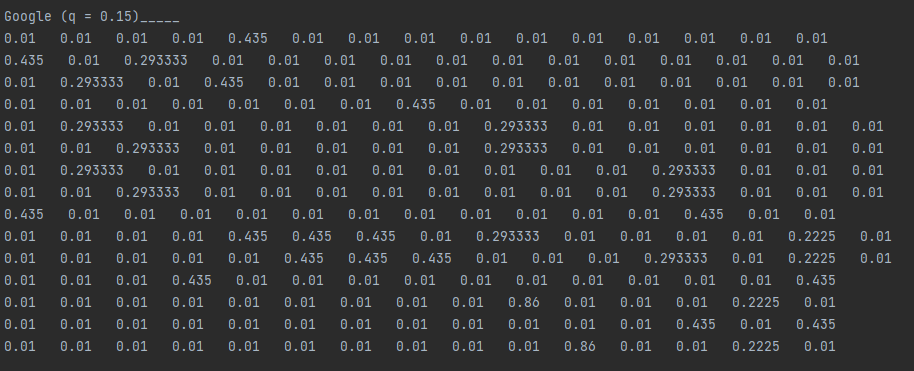
\includegraphics[scale=0.65]{images/google q = 0.15.png}        
\end{center}

%%ΠΡΩΤΟ ΖΗΤΟΥΜΕΝΟ ΤΕΤΑΡΤΗΣ ΑΣΚΗΣΗΣ
\textbf{\gt Ζητούμενο α)}\\
\gt Αθροίζουμε όλες τις στήλες του πίνακα \lt Google \gtκαι διαπιστώνουμε ότι όλες δίνουν
\gt αποτέλεσμα 1. Επομένως ο \lt Google \gtείναι στοχαστικός.\\

%%ΔΕΥΤΕΡΟ ΖΗΤΟΥΜΕΝΟ ΤΕΤΑΡΤΗΣ ΑΣΚΗΣΗΣ
\textbf{\gt Ζητούμενο β)}\\
\gt Εφαρμόζοντας τη μέθοδο των δυνάμεων για τυχαίο αρχικό διάνυσμα έως ότου
\begin{equation*}
    \left| \lambda ^{(m+1)} - \lambda ^{(m)}\right| < 0.5*10^{-7}
\end{equation*}
\gt (για ακρίβεια 7 δεκαδικών ψηφίων), \newpage
\gt έχουμε (κατά προσέγγιση) το ζητούμενο διάνυσμα:
\begin{equation*}
        \textbf{\lt p} = 
        \begin{bmatrix}
            0.0268246\\   
            0.0298611\\   
            0.0298611\\   
            0.0268246\\   
            0.0395872\\   
            0.0395872\\   
            0.0395872\\   
            0.0395872\\   
            0.0745644\\   
            0.10632\\   
            0.10632\\   
            0.0745644\\   
            0.125092\\   
            0.116328\\   
            0.125092\\ 
        \end{bmatrix}
    \end{equation*}\\
    
%%ΤΡΙΤΟ ΖΗΤΟΥΜΕΝΟ ΤΕΤΑΡΤΗΣ ΑΣΚΗΣΗΣ
\textbf{\gt Ζητούμενο γ)}\\
\gt Θα αυξήσουμε τον βαθμό σημαντικότητας της σελίδας 14.\\
\gt Καταργούμε την σύνδεση \lt14 \gtπρος 10 και προσθέτουμε τις\\\
\lt9,10,11,12 \gtπρος 14.\\
\gt Έτσι, από βαθμό σημαντικότητας
\begin{equation*}
    0.116328
\end{equation*}
\gt έχουμε μεταπήδηση σε
\begin{equation*}
    0.215643
\end{equation*}
\gt δηλαδή σχεδόν διπλασιασμό της σημαντικότητας της σελίδας 14\\

%%ΤΕΤΑΡΤΟ ΖΗΤΟΥΜΕΝΟ ΤΕΤΑΡΤΗΣ ΑΣΚΗΣΗΣ
\textbf{\gt Ζητούμενο δ)}\\
\gt Με την ίδια διαδικασία του ζητούμενου β) έχουμε τα καινούρια ιδιοδιανύσματα:
\begin{itemize}
    \item \textbf{\lt q = 0.02}
    \begin{equation*}
        \textbf{\lt p} = 
        \begin{bmatrix}
            0.0109388\\   
            0.0104914\\   
            0.0116267\\   
            0.0140127\\   
            0.0196029\\   
            0.0199738\\   
            0.0255053\\   
            0.0258762\\   
            0.0605812\\   
            0.0480659\\   
            0.142132\\   
            0.0846726\\   
            0.109975\\   
            0.260478\\   
            0.156067
        \end{bmatrix}
    \end{equation*}
    \item \textbf{\lt q = 0.6}
    \begin{equation*}
        \textbf{\lt p} = 
        \begin{bmatrix}
            0.0508324\\   
            0.0578847\\   
            0.057887\\   
            0.050845\\   
            0.054162\\  
            0.0541623\\   
            0.0542249\\   
            0.0542252\\   
            0.0644403\\   
            0.0789539\\   
            0.0946076\\   
            0.065069\\   
            0.071369\\   
            0.116837\\   
            0.0744998
        \end{bmatrix}
    \end{equation*}\\
\end{itemize}

\gt Παρατηρούμε ότι οι σελίδες με μεγάλη σημαντικότητα χάνουν βαθμό καθώς η πιθανότητα μεταπήδησης
\gt αυξάνεται και κερδίζουν βαθμό όταν μειώνεται, και το αντίθετο για τις σελίδες μικρής
\gt σημαντικότητας.

\gt Αυτό το συμπέρασμα είναι λογικό, αφού αν ο χρήστης έχει τάση να αλλάζει σελίδες συχνά τότε
\gt η σημασία της σημαντικότητας της σελίδας πέφτει, ενώ αν του αρέσει να μένει πολύ ώρα σε
\gt συγκεκριμένες σελίδες τότε η σημασία της σημαντικότητας των σελιδών αυξάνεται, καθώς αυτές
\gt έχουν μεγαλύτερη πιθανότητα να επιλεχτούν.

\gt Θα λέγαμε τελικά πως η πιθανότητα μεταπήδησης \lt q \gt χαρακτηρίζει
\textbf{\gt τη συμπεριφορά του χρήστη στο \lt Internet.}

\newpage
%%---------ΠΕΜΠΤΟ ΖΗΤΟΥΜΕΝΟ ΤΕΤΑΡΤΗΣ ΑΣΚΗΣΗΣ---------
\textbf{\gt Ζητούμενο ε)}\\

\gt Αυξάνουμε τις τιμές Α(8,11), Α(12,11) του πίνακα γειτνίασης σε 3.\\
\gt Εφαρμόζοντας για ακόμα μια φορά την μέθοδο των δυνάμεων στον (νέο) πίνακα \lt Google
\gt βλέπουμε πως η τάξη της σελίδας 11 μεταπηδά από
\begin{equation*}
    0.10632
\end{equation*}
\gt σε
\begin{equation*}
    0.145776
\end{equation*}

\gt Παρατηρούμε πως η τάξη όντως αυξάνεται, αλλά όχι δραστικά.

\gt Κάτι τέτοιο είναι λογικό να συμβαίνει, καθώς και να προβάλλει μια σελίδα μια άλλη με
\gt εξαιρετικό τρόπο, ο χρήστης, αν την επιλέξει, θα την επιλέξει μια φορά.
\gt Άρα η aξία της τιμής δεν έχει μεγάλη σημασία, άλλωστε από μαθηματικής άποψης
\gt ο πίνακας γειτνίασης νοιάζεται μόνο αν μια τιμή είναι μηδενική ή όχι (είναι πίνακας \lt Boole).

\gtΜπορούμε να συμπεράνουμε
\gt πως η τακτική αυτή δεν είναι τόσο καλή, σε σύγκριση με την τακτική του ζητούμενου γ).\\

\newpage
%%---------ΕΚΤΟ ΖΗΤΟΥΜΕΝΟ ΤΕΤΑΡΤΗΣ ΑΣΚΗΣΗΣ---------
\textbf{\gt Ζητούμενο στ)}\\

\gt Διαγράφουμε τον κόμβο 10, μικραίνοντας τον Α σε \lt 14x14.
\gt Καθώς το ιδιοδιάνυσμα συνεχίζει να αθροίζει σε 1, όλες οι τάξεις αλλάζουν:\\
\begin{center}
    \begin{tabular}{|p{6cm}|p{6cm}|}
        \hline
        \multicolumn{2}{|c|}{\gt Ιδιοδιάνυσμα \lt P}\\
        \hline
         \gt Πριν &  \gt Μετά\\
        \hline
            0.0268246 & 0.0427553\\
        \hline
            0.0298611 & 0.0369473\\
        \hline
            0.0298611 & 0.028454\\
        \hline
            0.0268246 & 0.0171089\\
        \hline
            0.0395872 & 0.0376954\\
        \hline
            0.0395872 & 0.0352889\\
        \hline
            0.0395872 & 0.0324987\\
        \hline
            0.0395872 & 0.0300922\\
        \hline
            0.0745644 & 0.0582801\\
        \hline
            0.10632 & N/A\\
        \hline
            0.10632 & 0.179915\\
        \hline
            0.0745644 & 0.0798776\\
        \hline
            0.125092 & 0.0691642\\
        \hline
            0.116328 & 0.206294\\
        \hline
            0.125092 & 0.145628\\
        \hline
    \end{tabular}
\end{center}
\newpage

\gt Παρατηρούμε πως στις σελίδες που έδειχναν προς την 10 αυξήθηκε η τάξη,
\gt ενώ σε αυτές που έδειχνε η 10 μειώθηκε η τάξη.

\gt Αναμενόμενο αποτέλεσμα, καθώς στην πρώτη περίπτωση οι σελίδες αυτές προσφέρουν
\gt λιγότερες επιλογές στον χρήστη για να τις εγκαταλείψει, ενώ στην δεύτερη περίπτωση
\gt υπάρχουν λιγότερες διαδρομές που οδηγούν στις σελίδες αυτές, και άρα λιγότερο \lt traffic.

\newpage
%%---------ΠΕΡΙΓΡΑΦΕΣ ΚΩΔΙΚΑ---------
\section{\gt Περιγραφές Κώδικα:}
\begin{itemize}
    \item \textbf{\gt Ασκήσεις 1 και 2:}\\
            \gtΣε όλες τις ζητούμενες μεθόδους γίνεται πρωτίστως έλεγχος του θεωρήματος
            \lt Bolzano \gt για το δοσμένο διάστημα. Στις διχοτομήσεις στην αρχή κάθε επανάληψης,
            \gt στις υπόλοιπες μόνο μια φορά, στην αρχή της διαδικασίας. Μετ'έπειτα εκτελείται
            \gt η ανάλογη κάθε φορά επαναληπτική πράξη, έως ότου να βρεθεί ρίζα στα άκρα του
            \gt δοσμένου διαστήματος ή το σφάλμα της προσέγγισης να γίνει ικανοποιητικά μικρό.
            
            \gtΟι αρχικοποιήσεις των επαναληπτικών διαδικασιών γίνονται πάντα βάση του δωσμένου
            \gtδιαστήματος. Στις διχοτομήσεις ορίζουν τα όρια του δείγματος, στις \lt Newton-Raphson
            \gtεπιλέγεται το κατάλληλο ώστε να ισχύει 
            \begin{equation*}
                f''(x_{0})f(x_{0}) > 0
            \end{equation*} 
            \gt και στις μεθόδους τέμνουσας χρησιμοποιούνται και τα 2, συν το μέσο
            \gt για την παραλλαγμένη της εκδοχή.
    \item \textbf{\gt Ασκήσεις 3 και 4:}\\
            \gt Για τις 2 αυτές ασκήσεις έχει δημιουργηθεί η κλάση \lt matrix, \gt μαζί με τις
            \gt υποκλάσεις τις \lt square\_matrix \gt και \lt column. \gt Οι κλάσεις αυτές
            \gt στηρίζονται στην \lt std::vector \gt και διευκολύνουν τις διαδικασίες, αφού δεν
            \gt χριάζεται έλεγχος αν ο πίνακας είναι πχ τετραγωνικός κλπ.
            
            \gt Έχοντας χτίσει αυτή τη βάση:
            \begin{itemize}
                \item [-] \textbf{\gt Άσκηση 3:}
                \begin{itemize}
                    \item [--] \textbf{\lt LU:}
                            \gt Δέχεται με αναφορά έναν τετραγωνικό πίνακα
                            \gt και επιστρέφει έναν πίνακα από \lt matrices L,U,P,
                            \gt οι αποσυνθέσεις του Α με βάση τη λογική \lt PA = LU
                    \item [--] \textbf{\lt Gauss:}
                            \gt Δέχεται με αναφορά έναν τετραγωνικό πίνακα και μία στήλη.
                            \gt Έλεχγει αν ο τετραγωνικός και η στήλη έχουν ίδιο μήκος και αν όχι,
                            \gt επιστρέφει \lt nullptr.
                            \gt Αν ναι, καλεί την \lt LU \gt και χρησιμοποιεί τα \lt returns
                            \gt για να λύσει το σύστημα:
                            \begin{equation*}
                                \begin{cases}
                                    Ly = Pb\\
                                    Ux = y
                                \end{cases}
                            \end{equation*} 
                    \item [--] \textbf{\lt Cholesky:}
                            \gt Δέχεται με αναφορά έναν τετραγωνικό πίνακα,
                            \gt ο οποίος σύμφωνα με την εκφώνηση θεωρείται συμμετρικός
                            \gt και θετικά ορισμένος. Βάση αυτού, χτίζει και επιστρέφει
                            \gt τον \lt L, \gt εκτελώντας τα παρακάτω:
                            \begin{equation*}
                                \begin{cases}
                                    L_{j,j} = \sqrt{A_{j,j} - \sum_{k=1}^{j-1}L_{j,k}^{2}}\\
                                    L_{i,j} = \frac{1}{L_{j,j}}(A_{i,j} - \sum_{k=1}^{j-1}L_{i,k}L_{j,k}) \quad i>j
                                \end{cases}
                            \end{equation*}
                    \item [--] \textbf{\lt Gauss-Seidel:}
                            \gt Δέχεται με αναφορά έναν τετραγωνικό πίνακα, μία στήλη
                            \gt και την ανοχή ε.
                            \gt Ελέγχει αν ο τετραγωνικός (Α) έχει κυριαρχική διαγώνιο και αν
                            \gt ο Α και η στήλη (\lt b) \gt έχουν ίδιο μήκος. Αν όχι, επιστρέφει
                            \lt nullptr.
                            \gt Αν ναι, αρχικοποιεί μια καινούρια στήλη \lt x \gt σε 0 και
                            \gt ξεκινά, από την θέση 0 και κάτω, να το ενημερώνει:
                            \begin{equation*}
                                x_{i} = \frac{1}{A_{i,i}}(b_{i} - \sum_{j=0,j \neq i}^{n}A(i,j)*x_{j})
                            \end{equation*}
                            \gt επειδή η ανανέωση των \lt xi \gtγίνεται σε
                            \lt loop time, \gt εξασφαλίζεται ότι χρησιμοποιούνται
                            \begin{equation*}
                                \begin{cases}
                                    x_{j}^{(m+1)}, \quad \lt j<i\\
                                    x_{j}^{(m)}, \quad \lt j>i
                                \end{cases}
                            \end{equation*}
                            \gtΗ ενημέρωση σταματά όταν επιτευχθεί
                            \begin{equation*}
                                \left|\left| x^{(m+1)} - x^{(m)} \right|\right|_{\infty} < \epsilon
                            \end{equation*}
                            \gt οπότε και επιστρέφεται το τελικό \lt x.
                            \end{itemize}
                \item [-] \textbf{\gt Άσκηση 4:}
                \begin{itemize}
                    \item [--] \textbf{\lt get\_google\_matrix:}
                            \gt Δέχεται με αναφορά τον πίνακα Α και την πιθανότητα μεταπήδησης \lt q
                            \gt και επιστρέφει τον συμπληρωμένο πίνακα \lt Google \gt με βάση τον
                            \gt τύπο της εκφώνησης.
                    \item [--] \textbf{\lt is\_stochastic:}
                            \gt Δέχεται με αναφορά έναν τετραγωνικό πίνακα. Για κάθε στήλη του,
                            \gt αθροίζει τα στοιχεία της, και άν βρει το άθροισμα διάφορο του 1,
                            \gt τερματίζει με \lt false \gt. Αν τα βρεί όλα 1, επιστρέφει \lt true.
                    \item [--] \textbf{\lt power\_method:}
                            \gtΔέχεται με αναφορά έναν τετραγωνικό πίνακα (τον \lt Google), 
                            \gt την ανοχή ε και μια μεταβλητή όπου θα αποθηκευτεί η μέγιστη
                            \gt ιδιοτιμή για επιστροφή. 
                            \gt Για να αποφευχθεί αρχικοποίηση σε ιδιοδιάνυσμα κάθετο
                            \gt στο κυρίαρχο, δημιουργεί \lt p \gt με τυχαίες συντεταγμένες.
                            \gt Έπειτα εκτελεί αλλεπάλληλα τα εξής
                            \begin{equation}
                                p = Gp
                            \end{equation}
                            \begin{equation}
                                \lambda^{(m)} = p_{1}\\
                            \end{equation}
                            \begin{equation}
                                p^{(i)} = \frac{p}{\lambda^{(m)}}
                            \end{equation}
                            \gt έως ότου 
                            \begin{equation*}
                                \left| \lambda^{(m+1)} - \lambda^{(m)}\right| < \epsilon
                            \end{equation*}
                            \gt όποτε και το τελικό \lt p \gt διαιρείται με το άθροισμα όλων των
                            \gt στοιχείων του για να κανονικοποιηθεί σε στοχαστικό και επιστρέφεται.
                \end{itemize}
            \end{itemize}   
            
\end{itemize}

%%---------EOF---------
\end{document}
